\section{Information Theory}%
\label{sec:information-theory}
\vspace{0.5cm}
\begin{figure}[h!]%
  \label{fig:info}
  \centering
  \fcolorbox{black}{white}{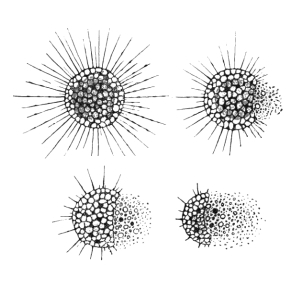
\includegraphics[width=0.3\textwidth]{entropy}}
  \caption{Visual representation of information entropy \href{https://www.consciousentities.com/2017/02/consciousness-entropy/}{(Conscious Entities, Peter Hankins)}}
\end{figure}
\vspace{0.5cm}

Information theory emerged in 1948 with Claude Shannon's seminal work \textit{A Mathematical Theory of Communication}. Shannon's framework, inspired by thermodynamics concepts from Boltzmann and Gibbs and communication theory from Hartley and Nyquist at Bell Labs~\cite{ref:losee-1997}, revolutionized our understanding of information quantification and transmission. While applications like data compression, error-correcting codes, and channel capacity are beyond this thesis's scope, we focus on information-theoretic quantities fundamental to machine learning and generative adversarial networks.

\begin{remark}
  In information theory, we quantify information about probability distributions rather than the semantic content of outcomes. Probability distributions capture our uncertainty about outcomes, making them central to information measurement. The most valuable information lies in accurately characterizing these distributions.
\end{remark}

Information theory provides essential tools for deep learning. Viewing neural networks as noisy channels highlights the relevance of information-theoretic principles. As David Mackay observed in~\cite{ref:mackay-2003}, ``brains are the ultimate compression and communication systems. And the state-of-the-art algorithms for both data compression and error-correcting codes use the same tools as machine learning.'' This symbiotic relationship suggests that advancing artificial intelligence methods will lead to better compression algorithms, and vice versa.

\subsection{Entropy: Quantifying Uncertainty}
The cornerstone of information theory is entropy, which measures uncertainty in probability distributions. We derive entropy by defining uncertainty as a function $\eta$ that satisfies intuitive requirements.

\begin{definition}
  Let $(\mathcal{X}, p)$ be a discrete probability space. We define \textnormal{\sffamily uncertainty} as a real-valued function $\eta(\cdot): \mathcal{X} \mapsto \mathbb{R}^+$ that depends only on outcome probabilities and satisfies:
  \begin{enumerate}[(i)]
  \item If outcome $x$ is certain, $\eta(x) = 0$ (no uncertainty);
  \item For outcomes $x, x'$, $p(x) < p(x') \iff \eta(x) > \eta(x')$ (rarer events are more surprising);
  \item For independent outcomes $x, x'$, $\eta(x \cdot x') = \eta(x) + \eta(x')$ (uncertainty is additive).
  \end{enumerate}
\end{definition}
\begin{remark}
  This definition adapts concepts from~\cite{ref:martin-2011} for our context.
\end{remark}

New information reduces uncertainty, with rare events providing more information than common ones. This suggests $\eta$ should be inversely proportional to probability:
\begin{align}
  \label{eq:eta-1}
  \eta(x) \propto {1 \over p(x)}
\end{align}

The additivity requirement (iii) implies a logarithmic relationship since independent events' probabilities multiply while their information content should add:
\begin{align}
  \label{eq:eta-3}
  \eta(x) = \log{1 \over p(x)}.
\end{align}

For a probability distribution, we need an average uncertainty measure weighted by outcome probabilities. This leads to entropy, denoted by $H$ (resembling the Greek eta):
\begin{align}
  \label{eq:eta-almost}
  H(p) = \sum_{x \in \mathcal{X}} p(x) \log{1 \over p(x)}.
\end{align}

Entropy represents the average surprise associated with outcomes from $(\mathcal{X}, p)$. It reaches maximum when all outcomes are equally likely (uniform distribution), reflecting maximum uncertainty:
\begin{align}
  \label{eq:eta-2}
  H(p) \leq \log{|\mathcal{X}|}
\end{align}

We can also interpret entropy as the average information (in bits) needed to describe outcomes from $(\mathcal{X}, p)$. The logarithm base determines the units:
\begin{align}
  \label{eq:understand-log}
  \log_2{1 \over p(x)} = n \iff 2^n = {1 \over p(x)}.
\end{align}
While base 2 yields bits, base $e$ (nats) and base 10 (dits) are also common.

\begin{definition}
  Let $(\mathcal{X}, p)$ be a discrete probability space. The \textnormal{\sffamily entropy} of distribution $p$ is:
  \begin{align}
    \label{eq:entropy}
    H(p) = - \mathbb{E}_{x \sim p} \left[ \log{p(x)} \right].
  \end{align}
  Entropy quantifies the average uncertainty in outcomes from $(\mathcal{X}, p)$. The uniform distribution maximizes entropy, as all outcomes are equally surprising.
\end{definition}

\begin{figure}[H]
  \centering
  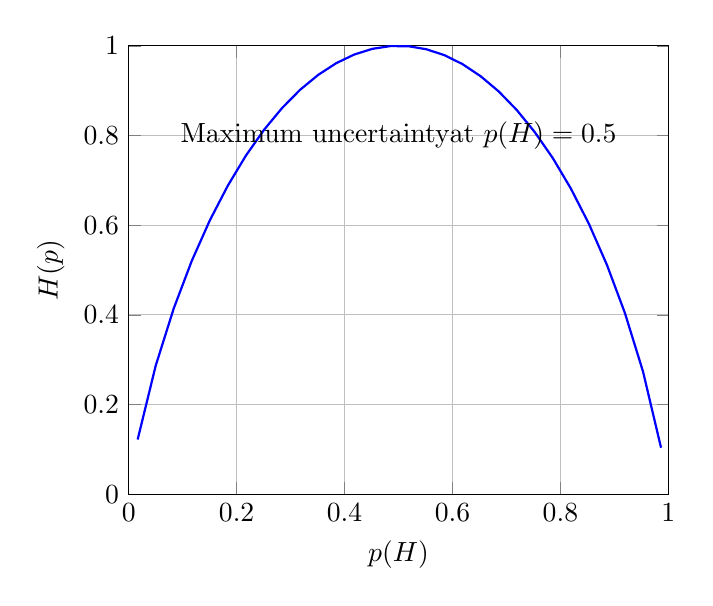
\begin{tikzpicture}
    \begin{axis}[
      ymin = 0,
      ymax = 1,
      xmin = 0,
      xmax = 1,
      xlabel = $p(H)$,
      ylabel = $H(p)$,
      enlargelimits = false,
      grid=major]
      \addplot [samples = 300, blue, thick] {-x*log2(x)-(1-x)*log2(1-x)};
      \node at (axis cs:0.5,0.8) {Maximum uncertainty\\at $p(H)=0.5$};
    \end{axis}
  \end{tikzpicture}
  \caption{Entropy of a coin toss as a function of the probability of heads $p(H)$. Entropy is maximized at 1 bit when the coin is fair ($p(H)=0.5$) and minimized at 0 when the outcome is certain ($p(H)=0$ or $p(H)=1$).}%
  \label{fig:entropy-coin-toss}
\end{figure}

\begin{example}
  The entropy of a fair coin toss is 1 bit. For $m$ independent fair tosses, entropy is $m$ bits. With three equally likely outcomes, entropy is $\log_2{3} \approx 1.585$ bits.
\end{example}

\subsection{Divergences and Distance Measures}
To compare probability distributions, we need measures of dissimilarity. We first distinguish between metrics and divergences.

\begin{definition}
  A \textnormal{\sffamily metric} on a set $\mathcal{X}$ is a function $d(\cdot, \cdot): \mathcal{X} \times \mathcal{X} \mapsto \mathbb{R}^+$ satisfying $\forall x, y, z \in \mathcal{X}$:
  \begin{enumerate}
  \item $d(x, y) \geq 0$, and $d(x, y) = 0 \iff x = y$ (non-negativity and identity)
  \item $d(x, y) = d(y, x)$ (symmetry)
  \item $d(x, z) \leq d(x, y) + d(y, z)$ (triangle inequality)
  \end{enumerate}
\end{definition}

\begin{remark}
  A divergence is a weaker notion than distance. It need not be symmetric nor satisfy the triangle inequality, but must be non-negative and zero only for identical distributions.
\end{remark}

\begin{definition}
  Let $\mathcal{P}$ be a space of probability distributions over finite set $\mathcal{X}$ with identical support. A \textnormal{\sffamily divergence} on $\mathcal{P}$ is a function $\text{D}(\cdot, \cdot): \mathcal{P} \times \mathcal{P} \mapsto \mathbb{R}^+$ such that $\forall p, q \in \mathcal{P}$:
  \begin{enumerate}[(i)]
    \item $\text{D}(p, q) \geq 0$
    \item $\text{D}(p, q) = 0 \iff p = q$.
  \end{enumerate}
\end{definition}

\subsubsection{Kullback-Leibler Divergence}
The most fundamental divergence in information theory is the Kullback-Leibler (KL) divergence.

\begin{definition}%
  \label{def:kl-divergence}
  The \textnormal{\sffamily Kullback-Leibler divergence} (also called \textnormal{\sffamily relative entropy}, \textnormal{\textsf directed divergence}, \textnormal{\sffamily information gain}, or \textnormal{\sffamily discrimination information}) between distributions $p$ and $q$ is:
  \begin{align}
    \label{eq:KL}
    \text{KL}(p \| q) = \sum_{x \in \mathcal{X}} p(x) \log{p(x) \over q(x)}.
  \end{align}
  If $p$ and $q$ have the same support, $\text{KL}(p \| q) = 0$ if and only if $p = q$.
\end{definition}

\begin{remark}
  KL divergence requires $p$ to be absolutely continuous with respect to $q$ ($q(x) = 0 \implies p(x) = 0$). When $p(x) = 0$, $\text{KL}(p \| q) = 0$ since $\lim_{x \to 0} x\log{x} = 0$.
\end{remark}

\begin{theorem}[Pythagorean Identity for KL Divergence]
  For a closed convex set $E \subset \mathcal{P}$ and distribution $Q \not \in E$, let $P^* \in E$ be the projection $p^* = \argmin_{P \in E} \text{KL}(p \| q)$. Then:
  \begin{align}
   \text{KL}(p \| q) \geq \text{KL}(p \| p^*) + \text{KL}(p^* \| q).
  \end{align}
  See Theorem 11.6.1 in~\cite{ref:cover-thomas} for details.
\end{theorem}

\begin{remark}
  KL divergence relates to the log-likelihood ratio test for comparing statistical models. For models $p(x) = f(x|\theta)$ and $q(x) = f(x|\phi)$, the log-likelihood ratio is:
  \begin{align}
    \lambda(x) & = \log{\prod_{x \in \mathcal{X}} p(x) \over \prod_{x \in \mathcal{X}} q(x)} = \sum_{x \in \mathcal{X}} \log {p(x) \over q(x)}
  \end{align}
  The KL divergence $\text{KL}(p \| q)$ is the expectation of $\lambda(x)$ under $p$:
  \begin{align}
    \mathbb{E}_{x \sim p}[\lambda(x)] = \sum_{x \in \mathcal{X}} p(x)\log {p(x) \over q(x)}.
  \end{align}
\end{remark}

This connection reveals that GAN training can be viewed as optimizing a goodness-of-fit test. The GAN objective:
\begin{align}
  \min_\phi\max_\theta{1 \over n} \sum_{i=1}^n \log{D_\theta(x_i)} + {1 \over n} \sum_{i=1}^n\log{(1 - D_\theta(G_\phi(z_i)))}
\end{align}
has the same fixed point as:
\begin{align}
  \min_\phi\max_\theta{1 \over n} \sum_{i=1}^n \log{\left({D_\theta(x_i) \over D_\theta(G_\phi(z_i))}\right)}
\end{align}
which represents a KL divergence or average log-likelihood ratio. Since $D_\theta(x) \in [0, 1]$, an optimal $D$ assigns higher probability to real data than generated data.

The term \textit{information gain} reflects that $\text{KL}(p \| q)$ quantifies information gained when using $q$ instead of $p$ to model data, or equivalently, information lost when $q$ approximates $p$.

\begin{definition}
  The \textnormal{\sffamily reverse Kullback-Leibler divergence} is:
  \begin{align}
    \label{eq:reverse-KL}
    \text{KL}(q \| p) = \sum_{x \in \mathcal{X}} q(x) \log{q(x) \over p(x)}.
  \end{align}
  This represents the expectation of the log-likelihood ratio under $q$:
  \begin{align}
    \mathbb{E}_{x \sim q}[\lambda(x)] = \sum_{x \in \mathcal{X}} q(x)\log {q(x) \over p(x)}.
  \end{align}
\end{definition}
Unlike forward KL, minimizing reverse KL is not equivalent to maximum likelihood estimation.

\subsubsection{Cross Entropy}
Cross entropy measures the average uncertainty when using $q$ to encode events from $p$.

\begin{definition}
  The \textnormal{\sffamily cross entropy} between $p$ and $q$ is:
  \begin{align}
    H(p, q) = - \sum_{x \in \mathcal{X}} p(x) \log q(x) = -\mathbb{E}_{x \sim p}\left[\log{q(x)}\right].
  \end{align}
  It represents the total uncertainty incurred by modeling data with $q$ instead of $p$.
\end{definition}

\begin{lemma}
  Cross entropy decomposes as $H(p, q) = H(p) + \text{KL}(p \| q)$.
\end{lemma}
\begin{proof}
\begin{align}
  H(p, q) & = -\sum_{x \in \mathcal{X}} p(x) \log q(x) \\
          & = -\sum_{x \in \mathcal{X}} p(x) \log p(x) + \sum_{x \in \mathcal{X}} p(x) \log p(x) - \sum_{x \in \mathcal{X}} p(x) \log q(x) \\
          & = -\sum_{x \in \mathcal{X}} p(x) \log p(x) + \sum_{x \in \mathcal{X}} p(x) \log {p(x) \over q(x)} \\
          & = H(p) + \text{KL}(p \| q)
\end{align}
\end{proof}

This decomposition shows cross entropy is bounded below by $H(p)$, with the excess quantified by $\text{KL}(p \| q)$. Cross entropy is asymmetric since $H(q, p) = H(q) + \text{KL}(q \| p)$.

\subsubsection{Jensen-Shannon Divergence}
The Jensen-Shannon divergence (JSD) provides a symmetric, smoothed version of KL divergence.

\begin{definition}%
  \label{def:jsd}
  For distributions $p(x)$ and $q(x)$ over space $\mathcal{X}$, the \textnormal{\sffamily Jensen-Shannon divergence} is:
  \begin{align}
    \text{JSD}(p \| q) = {1 \over 2} \text{KL}\left(p \| {p + q \over 2}\right) + {1 \over 2} \text{KL}\left(q \| {p + q \over 2}\right)
  \end{align}
\end{definition}

\begin{remark}
  JSD is the average of forward and reverse KL divergences with respect to the midpoint distribution $(p+q)/2$.
\end{remark}

\begin{theorem}
  The square root of Jensen-Shannon divergence, $\sqrt{\text{JSD}(p \| q)}$, is a metric.
\end{theorem}
\begin{proof}
  See~\cite{ref:endres-2003}.
\end{proof}

\subsection{Mutual Information and Dependency Measures}
Information theory provides tools to quantify dependencies between distributions.

\begin{definition}
  Let $(\mathcal{X}, p)$ and $(\mathcal{Y}, q)$ be finite probability spaces with random variables $X \sim p$ and $Y \sim q$. Their joint distribution is $\gamma$ with marginals $\pi_p \circ \gamma = p$ and $\pi_q \circ \gamma = q$. The \textnormal{\sffamily mutual information} $I(X;Y)$ is:
  \begin{align}
    \label{eq:mutual-information}
    I(X; Y) = \sum_{x \in \mathcal{X}}\sum_{y \in \mathcal{Y}}\gamma(x, y) \log{{\gamma(x, y) \over p(x)q(y)}}
  \end{align}
\end{definition}

\begin{theorem}
  If $X$ and $Y$ are independent, then $\gamma(x,y) = p(x)q(y)$ and $I(X; Y) = 0$.
\end{theorem}

\begin{remark}
  Mutual information quantifies the information shared between distributions, serving as a measure of statistical dependence. It can also be expressed as:
  \begin{align}
    \label{eq:mutual-information-alt}
    I(X; Y) = H(X) - H(X | Y) = H(Y) - H(Y | X)
  \end{align}
  where $H(X | Y)$ is the conditional entropy of $X$ given $Y$. This form shows mutual information as the reduction in uncertainty about one variable given knowledge of the other.
\end{remark}

\begin{figure}[h!]
  \centering
  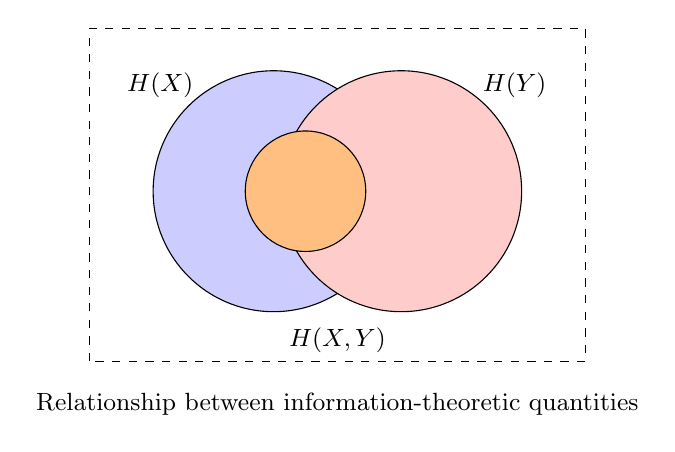
\begin{tikzpicture}[scale=0.9]
    \small
    % Labels
    \draw (0,0) node {$I(X;Y)$};
    \draw (-2.5,1.5) node {$H(X)$};
    \draw (2.5,1.5) node {$H(Y)$};
    \draw (-1.7,0) node {$H(X|Y)$};
    \draw (1.7,0) node {$H(Y|X)$};
    \draw (0,-2.1) node {$H(X,Y)$};
    % Circles
    \draw[fill=blue!20] (-0.9,0) circle (1.7cm);
    \draw[fill=red!20] (0.9,0) circle (1.7cm);
    % Intersection highlighting
    \draw[fill=orange!50] (-0.45,0) circle (0.85cm);
    % Bounding Rectangle
    \draw[dashed] (-3.5,-2.4) rectangle (3.5,2.3);
    % Caption
    \node at (0,-3) {Relationship between information-theoretic quantities};
  \end{tikzpicture}
  \caption{Venn diagram illustrating relationships between entropy $H(X)$, $H(Y)$, conditional entropy $H(X|Y)$, $H(Y|X)$, joint entropy $H(X,Y)$, and mutual information $I(X;Y)$.}%
  \label{fig:venn-information}
\end{figure}

\subsection{Information-Theoretic Analysis of GANs}%
\label{sec:info-value-function}%

We now analyze the GAN value function $V = \mathbb{E}_{x \sim p_r}[\log D_\theta(x)] + \mathbb{E}_{z \sim p_z}[\log(1 - D_\theta(G_\phi(z)))]$ from an information-theoretic perspective. The following proposition examines the optimization dynamics at each training step, while Section~\ref{sec:optimization-dynamics} analyzes limiting behavior.

GAN training aims to:
1. Minimize the KL divergence between the data distribution $p_r$ and the discriminator's output distribution $D_\theta(x)$
2. Maximize the KL divergence between the generator's prior $p_z$ and the discriminator's assessment of generated data $D_\theta(G_\phi(z))$
3. Minimize the KL divergence between $p_z$ and $D_\theta(G_\phi(z))$ from the generator's perspective

\begin{remark}
  KL divergence in this context quantifies the additional surprise when using an approximate distribution $q$ instead of the true distribution $p$.
\end{remark}

\begin{proposition}%
  \label{thm:info-objective}%
  The GAN objective:
  \begin{align}
    \label{eq:gan-objective}
    \min_\phi \max_\theta \mathbb{E}_{x \sim p_r}[\log D_\theta(x)] + \mathbb{E}_{z \sim p_z}[\log(1 - D_\theta(G_\phi(z)))]
  \end{align}
  corresponds to the following information-theoretic objectives:
\begin{enumerate}[(i)]
  \item Discriminator optimization: Find $\theta \in \Theta$ to minimize $\text{KL}(p_r \| D_\theta)$ and maximize $\text{KL}(p_z \| D_\theta \circ G_\phi)$
  \item Generator optimization: Find $\phi \in \Phi$ to minimize $\text{KL}(p_z \| D_\theta \circ G_\phi)$
  \end{enumerate}
\end{proposition}

\begin{proof}
  The first term of $V$ is the negative cross entropy between $p_r$ and $D_\theta$:
\begin{align}
  \label{eq:neg-cross-entropy}
  - H(p_r, D_\theta) = \sum_{x \in \mathcal{X}} p_r(x)\log(D_\theta(x)) = \mathbb{E}_{x \sim p_r} [\log(D_\theta(x))].
\end{align}
Maximizing this term minimizes cross entropy $H(p_r, D_\theta)$. Since:
\begin{align}
  H(p_r, D_\theta) & = H(p_r) + \text{KL}(p_r \| D_\theta),
\end{align}
and $H(p_r)$ is fixed, minimizing cross entropy requires minimizing $\text{KL}(p_r \| D_\theta)$, achieved when $D_\theta(x) = p_r(x)$.

The second term of (\ref{eq:gan-objective}) is:
\begin{align}
  \mathbb{E}_{z \sim p_z}[\log(1 - D_\theta(G_\phi(z)))] = \sum_{z \sim p_z} p_z(z) \log (1 - D_\theta(G_\phi(z)))
\end{align}
The discriminator maximizes this, equivalent to maximizing:
\begin{align}
  -\sum_{z \sim p_z} p_z(z) \log (D_\theta(G_\phi(z))),
\end{align}
which is the negative cross entropy between $p_z$ and $D_\theta \circ G_\phi$. Thus, $D_\theta$ maximizes $\text{KL}(p_z \| D_\theta \circ G_\phi)$, making $D_\theta(G_\phi(z))$ as different as possible from $p_z$.

Conversely, the generator minimizes the same term, equivalent to minimizing cross entropy between $p_z$ and $D_\theta \circ G_\phi$, which minimizes $\text{KL}(p_z \| D_\theta \circ G_\phi)$.
\end{proof}

This analysis reveals that the generator aims to make the discriminator's output on generated data as uninformative as random noise, while the discriminator tries to match its output distribution to the true data distribution while distinguishing generated data from noise.

\subsection{Optimization Dynamics and Limiting Behavior}%
\label{sec:optimization-dynamics}%

We now rigorously analyze GAN optimization dynamics. Let $\mathcal{X}$ be the data space with true distribution $p_r$, and $\tilde{\mathcal{X}}$ be generated data with distribution $p_g$ induced by generator $G_\phi$. Let $X \sim p_r$, $\tilde{X} \sim p_g$, and $Z \sim p_z$ (noise prior).

We consider three equivalent forms of the value function:
\begin{align}
  V(\phi, \theta)(X, Z) & = \mathbb{E}_{x \sim p_r}[\log D_\theta(x)] + \mathbb{E}_{z \sim p_z}[\log(1 - D_\theta(G_\phi(z)))] \\
  \tilde{V}(\phi, \theta)(X, \tilde{X}) & = \mathbb{E}_{x \sim p_r}[\log D_\theta(x)] + \mathbb{E}_{\tilde{x} \sim p_g}[\log(1 - D_\theta(\tilde{x}))] \\
  \mathcal{V}(U) & = \mathbb{E}_{u \sim p_U} [p_r(u) \log D_\theta(u) + p_g(u) \log(1 - D_\theta(u))]
\end{align}
where $U \subset \mathbb{R}^2$ contains pairs $(x, \tilde{x})$, and $p_U$ is the joint distribution over these pairs.

\begin{theorem}[Optimal Discriminator]%
 \label{theorem:minimax}
 For any fixed generator $G_\phi$, the optimal discriminator $D^*$ that maximizes $V$ is:
  \begin{align}
    D^*(x) = \frac{p_r(x)}{p_r(x) + p_g(x)}.
  \end{align}
\end{theorem}
\begin{proof}
  We compute the derivative of $\mathcal{V}$ with respect to $\theta$:
  \begin{align}
    \label{eq:derivatives}
    {\partial \mathcal{V}(U) \over \partial \theta} = \mathbb{E}_{u \sim p_U}\left[ p_r(u) { {\partial D_\theta(u) \over \partial \theta} \over D_\theta(u)} - p_g(u) {{\partial D_\theta(u) \over \partial \theta} \over (1 - D_\theta(u))}\right],
  \end{align}
  Setting this to zero yields:
  \begin{align}
    \label{eq:20}
    {p_r(u) \over D_\theta(u)} = {p_g(u) \over (1 - D_\theta(u))} \iff D^*(u) = {p_r(u) \over p_g(u) + p_r(u)}.
  \end{align}
  Thus, for any fixed $G_\phi$, $\mathcal{V}(U)$ is maximized when $D_\theta = D^*$.
\end{proof}

Substituting $D^*$ into $\tilde{V}$ gives:
\begin{align}
  \label{eq:sum-of-two-kl-divergences}
   \max_D \tilde{V}(\phi, \theta)(X, \tilde{X}) = \mathbb{E}_{x \sim p_r}\left[\log{p_r(x) \over p_g(x) + p_r(x)}\right] + \mathbb{E}_{\tilde{x} \sim p_g}\left[\log{p_g(\tilde{x}) \over p_g(\tilde{x}) + p_r(\tilde{x})} \right]
\end{align}
This expression relates to the Jensen-Shannon divergence between $p_r$ and $p_g$.

\begin{lemma}
  The minimax value of the GAN game is $-\log 4$.
\end{lemma}
\begin{proof}
  The optimal generator satisfies $p_g = p_r$. Substituting into (\ref{eq:sum-of-two-kl-divergences}):
  \begin{align}
    V(\phi^*, \theta^*)(X, \tilde{X}) & = \mathbb{E}_{x \sim p_r}\left[\log{p_r(x) \over 2p_r(x)}\right] + \mathbb{E}_{\tilde{x} \sim p_r}\left[\log{p_r(\tilde{x}) \over 2p_r(\tilde{x})}\right] \\
                      & = \mathbb{E}_{x \sim p_r}[\log(1/2)] + \mathbb{E}_{\tilde{x} \sim p_r}[\log(1/2)] \\
                      & = -\log 2 - \log 2 = -\log 4
  \end{align}
\end{proof}

\begin{theorem}[GAN Optimization as JSD Minimization]%
  \label{thm:limiting}
  With an optimal discriminator, minimizing $V$ with respect to $\phi$ is equivalent to minimizing the Jensen-Shannon divergence between $p_r$ and $p_g$.
\end{theorem}
\begin{proof}
  Adding and subtracting $\log 4$ from (\ref{eq:sum-of-two-kl-divergences}) yields:
  \begin{align}
    \label{eq:desired}
    V(\phi, \theta^*) = 2 \cdot \text{JSD}(p_r \| p_g) - \log 4,
  \end{align}
  as shown in Appendix~\ref{sec:proof-for-jsd-thing}. Minimizing $V$ thus minimizes $\text{JSD}(p_r \| p_g)$.
\end{proof}

\subsection{Discussion}
This section presented two complementary information-theoretic perspectives on GAN training. Theorem~\ref{thm:limiting} characterizes the limiting behavior, showing that GAN optimization minimizes Jensen-Shannon divergence between real and generated distributions. Theorem~\ref{thm:info-objective} examines the optimization dynamics at each training step, revealing how the discriminator and generator alternately minimize and maximize Kullback-Leibler divergences.

The analysis shows that GANs avoid limitations of traditional maximum likelihood methods, which minimize forward KL divergence $\text{KL}(p_r \| p_g)$. This divergence is sensitive to mode dropping, as it penalizes generating samples where $p_g > 0$ but $p_r = 0$. In contrast, JSD provides a more balanced measure of distributional similarity.

During training, the discriminator progressively forces the value function to better approximate JSD by performing the operations in Theorem~\ref{thm:info-objective}. This stepwise optimization reveals the intricate interplay between discriminator and generator as they jointly minimize distributional divergence through adversarial dynamics.

%%% Local Variables:
%%% mode: latex
%%% TeX-master: "../thesis.tex"
%%% End:
